\section{Multiple Sources}\label{sect:super}
\begin{minipage}[l]{0.6\linewidth}
\hspace*{0.5in} 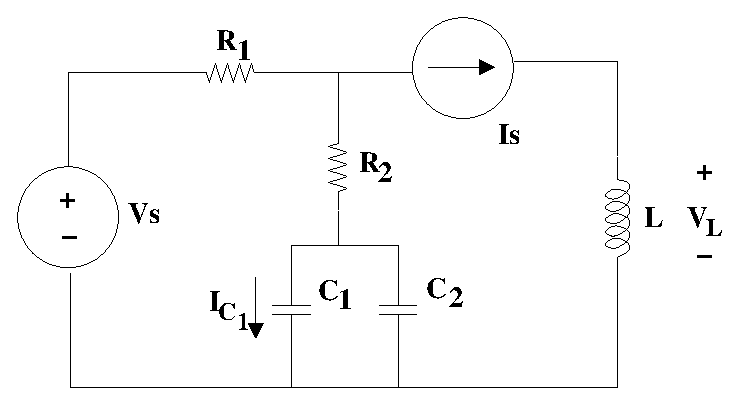
\includegraphics[width=0.7\linewidth]{superposition/superposition}
\end{minipage}\hfill
\begin{minipage}[l]{0.4\linewidth}
$V_s(t) = 20 \cos(100t)$ V\\ 
$I_s(t) = 10 \cos(1000t+20^\circ)$ mA\\
$R_1$ = 100 $\Omega$\\
$R_2$ = 500 $\Omega$\\ 
$C_1$ = 250 $\mu$F\\ 
$C_2$ = 750 $\mu$F\\ 
$L$ = 5 mH\\
\end{minipage}

Assume that all of the sources have been on for a long time (i.e., the circuit
is in a steady-state condition).

\begin{enumerate}
    \item Solve for an expression for $V_L(t)$.  \\
    \item Solve for an expression for $I_{C_1}(t)$. \\
\end{enumerate}
